\begin{frame}{preventing shadow stack writes?}
\begin{itemize}
\item ARM64 scheme: prevent writes if
    \begin{itemize}
    \item shadow stack pointer is never leaked (dedicated register)
    \item shadow stack random location can't be guessed (or queried otherwise)
    \end{itemize}
\item Intel CET: prevent writes unless
    \begin{itemize}
    \item OS (priviliged/kernel mode) instructions to setup shadow stack used
    \end{itemize}
\vspace{.5cm}
\item can we prevent writes without relying on avoiding info leaks\ldots \\
      and without special hardware support?
      \begin{itemize}
      \item well, yes, but \ldots
      \end{itemize}
\end{itemize}
\end{frame}

\begin{frame}{some early stack canary benchmarks}
{\small from Chiueh and Hsu, ``RAD: A Compile-Time Solution to Buffer Overflow Attacks'' (2001)}
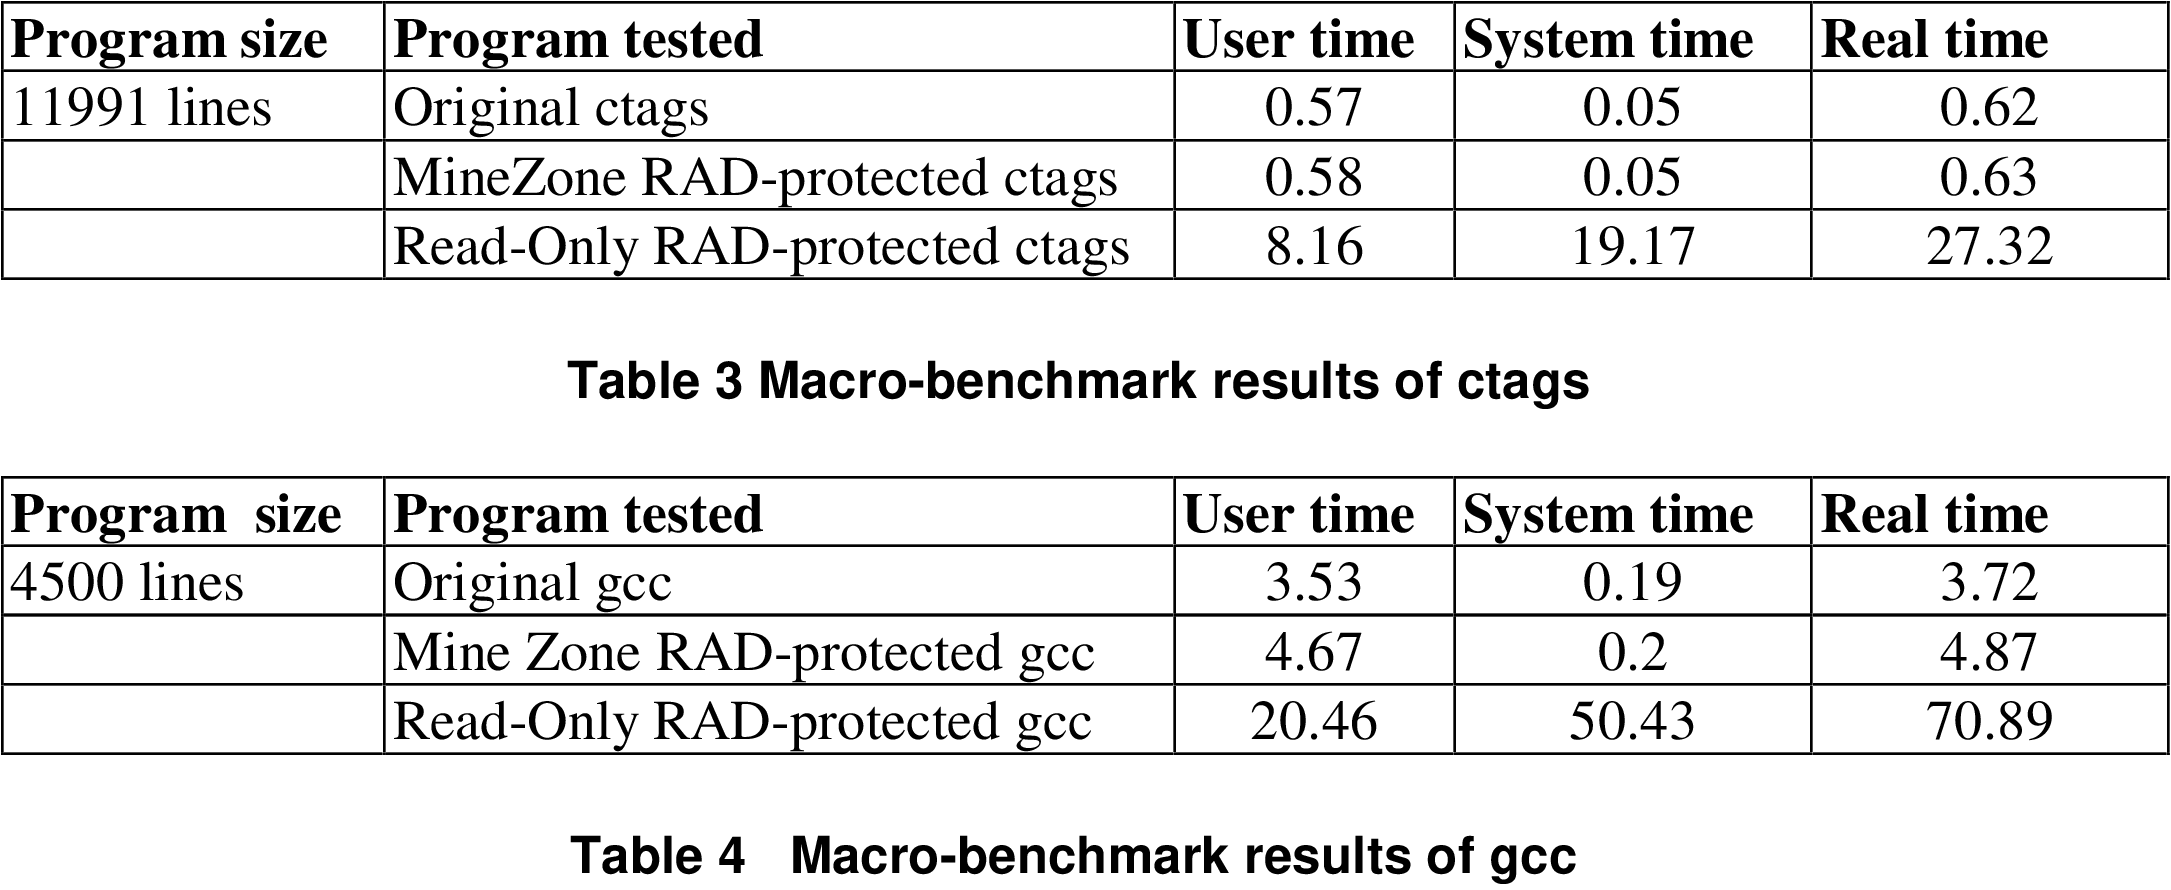
\includegraphics[height=0.8\textheight]{../mitigate/rad-results}
\end{frame}

